\documentclass[10pt]{report}

\usepackage{stan-talks}

\renewcommand{\baselinestretch}{1.05}

\newcommand{\drw}[2]{#1^{(#2)}}

\begin{document}
\sf%
\vspace*{-12pt}
%
\noindent
\spc{\Huge\bfseries \color{MidnightBlue}{WALNUTS:}}
\\[12pt]
\spc{\LARGE\bfseries \color{MidnightBlue}{Per-leapfrog step size
    adaptation for HMC}}
\\[16pt]
\noindent
\spc{\Large\bfseries \color{MidnightBlue}{Bob Carpenter}}
\\[8pt]
\spc{\large Center for Computational Mathematics}
\\[4pt]
\spc{\large Flatiron Institute}
\\[12pt]
\vfill
\hfill

\includegraphics[height=0.35in]{img/fi-logo.png}
\qquad

\includegraphics[height=0.5in]{img/stan-logo.png}

\sld{Bayesian statistics with Monte Carlo}
\begin{itemize}
\item Bayesian \myemph{posterior inference} given data $y$ with parameters $\theta$:
\[
\begin{array}{rrlr}
  \widehat{\theta} & = & \mathbb{E}[\Theta \mid y]
                         & \textrm{[parameter estimates]}
  \\[4pt]
  \null \Pr[E \mid y] & = & \mathbb{E}[\textrm{I}_E(\Theta) \mid y]
                            & \textrm{[event probability estimates]}
  \\[4pt]
  \null p(\widetilde{y} \mid y) & = & \mathbb{E}[p(\widetilde{y} \mid
                                      \Theta) \mid y]
              & \textrm{[posterior predictive density]}                                      
\end{array}
\]
\item Expectations involve \myemph{high-dimensional integrals}.
  $$\textstyle \mathbb{E}[f(\Theta) \mid y] = \int_\Theta f(\theta) p(\theta
  \mid y) \textrm{d}\theta. $$
\item (Markov chain) \myemph{Monte Carlo solves integrals} with $\theta^{(m)} \sim p(\theta \mid y).$
  $$\textstyle \mathbb{E}[f(\Theta) \mid y] \approx \frac{1}{M} \sum_{m=1}^M
  f(\theta^{(m)}) $$
\end{itemize}

\sld{Why NUTS?}
%
\begin{itemize}
\item Hamiltonian Monte Carlo (HMC, 1985), a Markov chain Monte
  Carlo (MCMC) method that \myemph{scales well in dimension}.
  \begin{subitemize}
  \item \myemph{integrated autocorrelation time}$^*$: $\mathcal{O}\left(D^{1/4}\right)$ \qquad \myemph{memory}: $\mathcal{O}(D)$
    \\ \qquad $^*$: times ``constant'' based on condition number (Langmore et al.\ 2020)
 \item Hamiltonian \myemph{gradient flow} overcomes diffusive random walk behavior.
  \end{subitemize}
\item Why wasn't HMC in wide use until the \myemph{no-U-turn sampler}
  (NUTS, 2012)?
  \vspace*{-8pt}
  \begin{subitemize}
  \item NUTS in Stan, PyMC, NumPyro, Turing.jl, Blackjax, NIMBLE, ADMB, etc.
  \end{subitemize}
  \vfill
\item \myemph{Double whammy}:
  \begin{subitemize}
  \item HMC is hard to tune; NUTS brought \myemph{self tuning} and \myemph{general software}.
  \item gradients are hard for applications; \myemph{automatic differentiation} makes it easy.
  \end{subitemize}
\end{itemize}

\sld{What is HMC and why is it hard to tune?}
\begin{itemize}
\item Fictitious physical system with \myemph{position} $\theta \in
  \mathbb{R}^D$ and \myemph{momentum} $\rho \in \mathbb{R}^D$:
  \begin{subitemize}
  \item \myemph{Potential} energy: $U(\theta) = - \log p(\theta)$ for
    \myemph{target density} $p(\theta)$
  \item \myemph{Kinetic} energy: $K(\rho) - \log \textrm{normal}(\rho \mid 0, M)$
  \item \myemph{Hamiltonian} (total energy): $H(\theta, \rho) =
    U(\theta) + K(\rho)$, \quad $p(\theta, \rho) = \exp\left( -H(\theta, \rho)\right)$
  \end{subitemize}
\item \myemph{HMC iteration} from position $\theta(0)$:
  \begin{subitemize}
  \item \myemph{Sample momentum}: $\rho(0) \sim \textrm{normal}(0, M)$
  \item \myemph{Evolve Hamiltonian exactly}: $(\theta(0), \rho(0))$ 
    to $(\theta(t), \rho(t))$, return $\theta(t)$.
  \end{subitemize}
\item In practice, can't solve exactly, so discretize.
  \begin{subitemize}
  \item \myemph{Simulate:} Take $L$ leapfrog steps of size $\epsilon = t / L$
    to $(\theta'(t), \rho'(t)) \approx (\theta(t), \rho(t))$.
  \item \myemph{Metropolize:} Return $\theta'(t)$ with probability $1 \wedge \frac{p(\theta'(t), \
      \rho(t)')}{p(\theta(0), \ \rho(0))}$; else return $\theta(0)$.
  \end{subitemize}
\end{itemize}

\sld{Harmonics in HMC}

\begin{minipage}[t]{0.7\textwidth}
  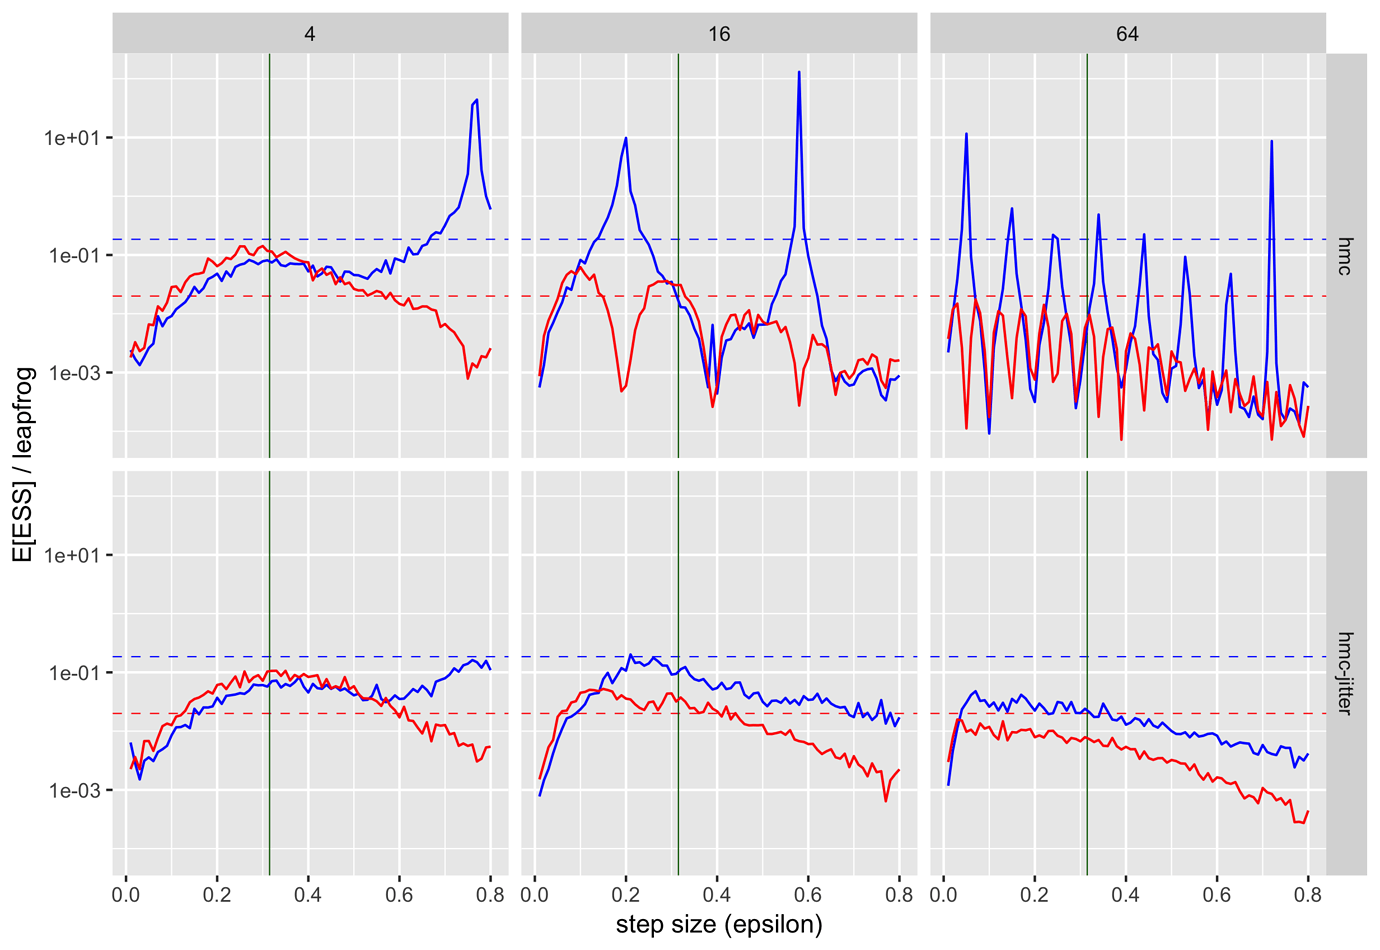
\includegraphics[width=\textwidth]{img/ess-per-leapfrog-jitter-hmc.png}
\end{minipage}%
\begin{minipage}[t]{0.29\textwidth}
  \null\vspace*{-2.5in}
  \begin{subitemize}
  \item \myemph{Target}: 1000-dim standard normal
  \item \myemph{y-axis} (log):  ESS; \\ \myemph{x-axis}: step size
  \item \myemph{blue}: $\mathbb{E}[\Theta]$; \\ \myemph{red}:
    $\mathbb{E}[\Theta^2]$
  \item \myemph{top}: HMC; \\ \myemph{bottom}: jittered time HMC
  \item \myemph{solid}:~HMC,\\ \myemph{dashed}: NUTS
  \end{subitemize}
\end{minipage}

\sld{Leapfrog integrator simulates trajectories}
\begin{itemize}
\item \myemph{Leapfrog step} from $(\theta(t), \rho(t))$ with step $\epsilon$, mass $M$
  \begin{eqnarray*}
    \rho(t + 1/2) & = & \rho(t) + \epsilon / 2 \cdot \nabla \log p(\theta(t))
    \\[4pt]
    \theta(t+1) & = & \theta(t) + \epsilon \cdot M^{-1} \cdot \rho(t + 1/2)
    \\[4pt]
    \rho(t + 1) & = & \rho(t + 1/2) + \epsilon / 2 \cdot \nabla \log p(\theta(t + 1)) 
  \end{eqnarray*}
\item \myemph{Stable} if $\epsilon < 2 / \sqrt{\lambda^\text{max}}$, where $\lambda^\textrm{max}$ is max eigenvalue of Hessian,
  $$H(\theta) = \nabla \nabla^\top \! -\log p(\theta)$$
  \begin{subitemize}
  \item \myemph{local error}:  $\mathcal{O}(\epsilon^3)$
  \item \myemph{global error}: $\mathcal{O}(\epsilon^2)$
  \end{subitemize}
\end{itemize}

\sld{Multinomial HMC}
\begin{itemize}
\item \myemph{Each iteration} from previous position $\theta(0)$:
  \begin{subitemize}
  \item generate new momentum $\rho(0) \sim \textrm{normal}(0, M)$
  \item generate \myemph{random steps forward} $F \sim \textrm{uniform}(\{ 0, \ldots, L \})$
  \item take $B = L - F$ leapfrog \myemph{steps backward} and $F$ forward from
    $(\theta(0), \rho(0))$
  \item yields $(\theta(n), \rho(n))$ for $-B \leq n \leq F$
    (including initial)
  \item \myemph{randomly select next state} $(\theta(n), \rho(n))$ \\[4pt]
    with probability \myemph{proportional to density}, $\null \propto p(\theta(n), \rho(n))$
  \end{subitemize}
\item \myemph{No rejection}, \myemph{no harmonics}, and \myemph{no bad
    luck} due to error $\pm H(\theta(0), \rho(0))$
  \vfill
\item Straightforward to prove \myemph{detailed balance} (cf. our
  second \textit{GIST} paper)
\end{itemize}

\sld{Naive no-U-turn sampler (NUTS)}
\begin{itemize}
\item Go forward or backward uniformly at random,
\item doubling number of steps each time,
\item until there is a U-turn between ends (i.e., ends heading toward each other).
\item But, if there is a sub-U-turn in the new states, throw away new doubling.
  \begin{subitemize}
  \item inefficient, but necessary for detailed balance
  \end{subitemize}
\item select next state proportional to density (a la multinomial HMC)
  \vfill
\item Original naive NUTS: slice sample rather than multinomial sample
\end{itemize}

\sld{Biased-progressive NUTS}
\begin{itemize}
\item Keep a selected state, initially $z(0) = (\theta(0), \rho(0))$
\item At each doubling from $M$ to $2M$ states:
  \begin{subitemize}
    \item Extend $z(1), \ldots, z(M)$ to $z(1), \ldots, z(M), z(M+1), \ldots, z(2M)$
    \item Metropolis \myemph{probability of updating state}:
      $$
      1 \wedge
      \dfrac{p\!\left(z(M+1)\right) + \cdots + p\!\left(z(2M)\right)}
            {p\!\left(z(1)\right) + \cdots + p\!\left(z(M)\right)}
            $$
          \item If Hamiltonian simulation perfect, probability is 1.            
      \item If updating, \myemph{select new state} $z(m)$ 
        with probability \myemph{proportional to density},  $\propto p(z(m))$,
        from among candidate states $z(M+1), \ldots, z(2M)$.
  \end{subitemize}
\item Return final selected item.
\end{itemize}

\sld{Biased-progressive vs. naive jump distance}
\begin{center}
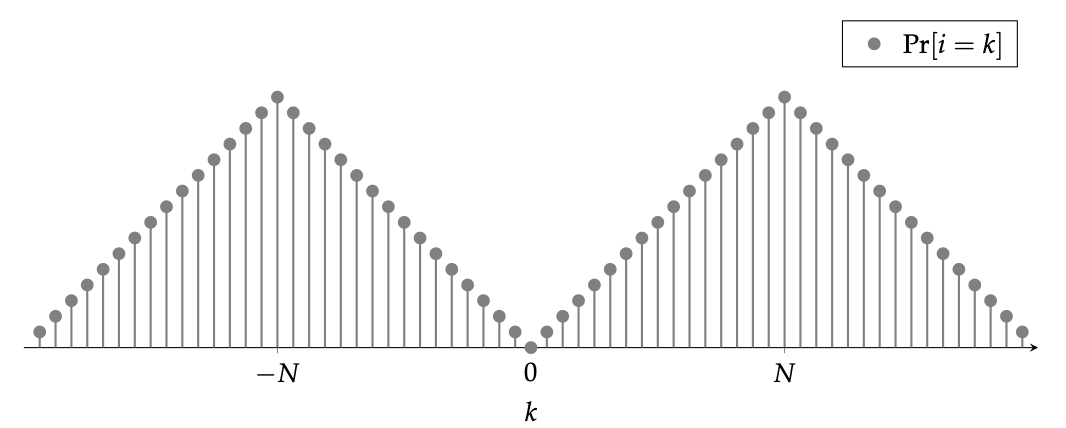
\includegraphics[width=0.6\textwidth]{img/multinomial-hmc-L.png}
\end{center}
\begin{itemize}
\item Assuming \myemph{perfect simulation} of the Hamiltonian trajectory, each state equally likely.
\item \myemph{Naive} NUTS and multinomial sample \myemph{uniformly} along trajectory.
\item \myemph{Biased-progressive} NUTS samples \myemph{as above} ($N = 2^M$ total steps)
\end{itemize}

\sld{Preconditioning with a mass matrix}
\begin{itemize}
\item The positive-definite \myemph{mass matrix} $M$ acts as a \myemph{global preconditioner}
\item If $\Theta \sim \textrm{normal}(\mu, \Sigma)$, then $M = \Sigma^{-1}$ is a \myemph{perfect preconditioner}
  \begin{subitemize}
  \item i.e., mass-adjustment samples like standard normal
  \end{subitemize}
\item NUTS uses \myemph{fixed warmup iterations} with unit mass matrix before sampling to estimate $\textrm{cov}[\Theta]$
\item \myemph{Chicken-and-egg} problem:
  \begin{subitemize}
  \item need to sample efficiently to estimate mass matrix effectively
  \item need good mass matrix to sample efficiently
  \end{subitemize}
\item There are \myemph{better mass matrix estimators} than we used for Stan (see below).
\end{itemize}

\sld{The curse of varying geometry}
\begin{itemize}
\item If the Hessian varies, \myemph{global preconditioning fails}.
  \begin{subitemize}
  \item e.g., \myemph{Neal's funnel}: condition varies 0 to 1000+,
    eigenstructure varies
  \end{subitemize}
\item By \myemph{adjusting step size} lower in neck (color), \myemph{WALNUTS succeeds}\\[12pt]
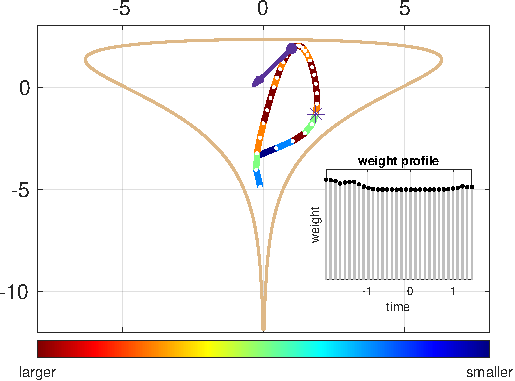
\includegraphics[width=0.32\textwidth]{img/funnel1.pdf}%
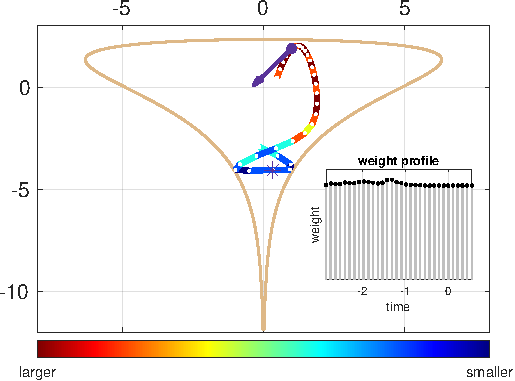
\includegraphics[width=0.32\textwidth]{img/funnel2.pdf}%
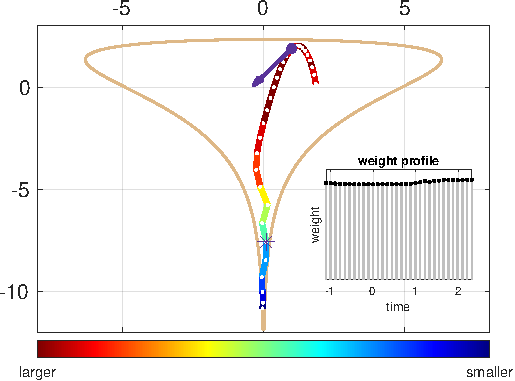
\includegraphics[width=0.32\textwidth]{img/funnel3.pdf}
\end{itemize}

\sld{Gibbs self tuning (GIST)}
\begin{itemize}
\item Couple \myemph{auxiliary tuning} variables to position/momentum
  \begin{subitemize}
  \item e.g., $\alpha = L, \epsilon, M$ (number of steps, step size, mass
    matrix) for HMC
    \end{subitemize}
\item \myemph{Gibbs sample} tuning parameters given state $\alpha \sim p(\alpha \mid \theta, rho)$
  \begin{subitemize}
  \item free to choose reasonable conditional distribution
  \end{subitemize}
\item Use tuning parameters $\alpha$ with NUTS to \myemph{propose} $\theta(t), \rho(t)$
\item Accept probability:
  $
  \Pr[\textrm{accept } \theta(t), \rho(t)]
  = \dfrac{p(\theta(t), \rho(t))}{\underbrace{p(\theta(0), \rho(0))}_\textrm{Metropolis}}
    \cdot 
    \dfrac{p(\alpha \mid \theta(t), \rho(t))}{\underbrace{p(\alpha \mid \theta(0), \rho(0))}_\textrm{correction}}
    $
\item {\small Bou-Rabee, N., Carpenter, B., and
    M. Marsden. 2024. \myemph{GIST: Gibbs self-tuning for locally adaptive
    Hamiltonian Monte Carlo}.
    {\slshape arXiv}:2404.15253.}
\end{itemize}

\sld{GIST II}
\begin{itemize}
\item We applied GIST to step size tuning (Bou-Rabee, Marsden, Kleppe, me)
\item Start at step size $\epsilon = \epsilon^\textrm{max}$
\item While selecting steps $L$ w.\ NUTS doesn't preserve Hamiltonian within $\tau$ between any two states on trajectory
  \begin{subitemize}
  \item $\epsilon = \epsilon / 2$
    \end{subitemize}
  \item \myemph{Correction is 1} if same number of halvings forward and backward; else reject.
    \vspace*{-12pt}
    \begin{subitemize}
    \item GIST technically allows further randomization around halvings.
    \end{subitemize}
  \vfill
  \item {\small Bou-Rabee, N., Carpenter, B., Kleppe, T.S. and
      Marsden, M., 2025. \myemph{Incorporating local step-size
        adaptivity into the No-U-Turn Sampler using Gibbs self
        tuning}. \textit{Journal of Chemical Physics}.}
\end{itemize}

\sld{GIST III: WALNUTS}
\begin{itemize}
\item Just like GIST II, but \myemph{adjust every leapfrog step}
  \begin{subitemize}
    \item accept correction is product of local corrections
  \end{subitemize}
\begin{center}
  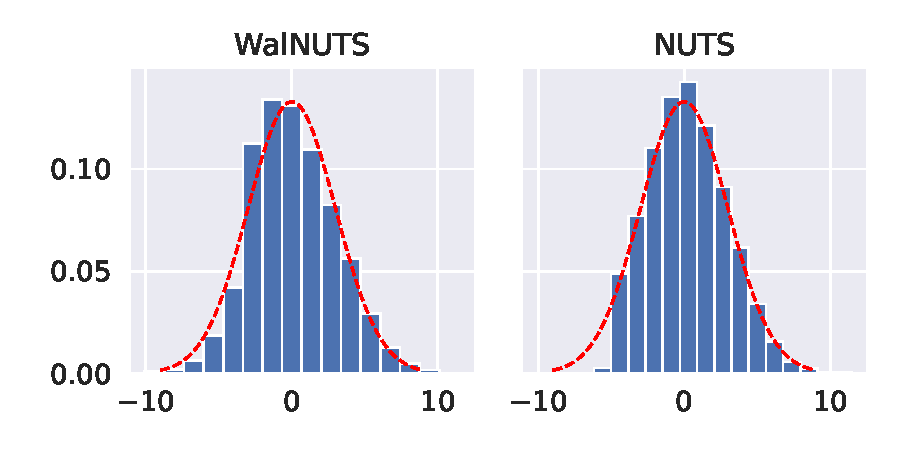
\includegraphics[width=0.55\textwidth]{img/funnel_hist.pdf}
\end{center}
\item {\small \myemph{Et voila!}}---this is log scale in Neal's funnel
  (marginal $\textrm{normal}(0, 3)$)
\end{itemize}


\sld{GIST for mass-matrix estimation}
\begin{itemize}
\item \myemph{Local mass matrix} adaptation.
\item For \myemph{log concave} can use GIST with inverse Wishart
  distribution around negative Hessian of log density
  \begin{subitemize}
  \item degrees of freedom determined by variability of Hessians
  \end{subitemize}
\item \myemph{Low rank plus diagonal} reduces
  $\mathcal{O}(N^3)$ to $\mathcal{O}(K^2 N)$.
\item Black-box Riemannian HMC tunes locally based on
  (positive-definite conditioned) Hessian
  \begin{subitemize}
  \item Implicit integrators $\mathcal{O}(N^3)$ and hard to tune
  \item Explicit interators only require $\mathcal{O}(N^2)$
    Hessian-vector products, but just as hard to tune
  \end{subitemize}
\end{itemize}

\sld{Nutpie-style mass matrix estimation}
\begin{itemize}
\item WALNUTS needs: \myemph{static mass matrix} and \myemph{static macro step size}
\item \myemph{Nutpie} (from Adrian Seyboldt of PyMC Labs) is state of
  the art
\item Mass matrix $M$ chosen to minimize \myemph{Fisher divergence}
  from preconditioned density to a standard normal
  $$
  \widehat{M} = \textrm{arg min}_M \textrm{D}_F[q_M \, || \,
  \textrm{normal}(0, 1)],
  $$
  where $q_M$ is target density preconditioned with $M$
\item Fisher divergence measures \myemph{gradient discrepancy},
  $$
  \textrm{D}_F[q \, || \, p] =
  \int_{\mathbb{R}^D} q(\theta) \cdot || \nabla \log q(\theta) - \nabla \log
  p(\theta)||^2_2 \ \textrm{d}\theta.
  $$
\end{itemize}

\sld{Minimizing Fisher divergence given draws}
\begin{itemize}
\item Same approach across \myemph{matrix forms}: diagonal, low-rank
  plus diagonal, dense
\item Geometric mean of inverse covariance of draws and covariance of
  scores
  \begin{subitemize}
    \item \myemph{score function}: $S(\theta) = \nabla \log
      p(\theta)$
    \item \myemph{motivation}: $\Theta \sim \textrm{normal}(\mu,
      \Sigma)$ implies
      $\textrm{cov}(\Theta) = \textrm{cov}^{-1}(S(\Theta)) = \Sigma$
    \item \myemph{Geometric mean} is midpoint of geodesic in \myemph{affine-invariant Riemannian manifold}
      (AIRM) of symmetric positive-definite matrixes
      \end{subitemize}
\item \myemph{Much faster to converge} than using only draws (e.g., NUTS)
\end{itemize}

\sld{Details of Fisher information minimization}
\begin{itemize}    
\item Suppose a \myemph{block of approximate draws} gathered during warmup
  $$\drw{\theta}{1:N} = \drw{\theta}{1}, \ldots,
  \drw{\theta}{N} \sim p(\theta)$$ 
\item Nutipe \myemph{estimates mass matrix} as
  $$
  \widehat{M} = \textrm{cov}^{-1}\!\left(\drw{\theta}{1:N}\right)
                \, \# \ 
                \textrm{cov}\!\left(S(\drw{\theta}{1:N})\right),
                $$
\item \myemph{AIRM geometric mean}: $A \, \# \, B = A^{1/2} \left( A^{-1/2} \, B \,
          A^{-1/2}\right)^{1/2} \, A^{1/2}$
        \begin{subitemize}
        \item \myemph{diagonal case}: $A \# B = (A \cdot B)^{1/2}$
          applied elementwise
          \end{subitemize}
\item Nutpie takes overlapping blocks of $N = 100$ draws
\end{itemize}

\sld{Fisher vs.\ variance-based mass matrices}
\begin{subitemize}
  \item Fisher outperforms covariance by median factor 1.3 over 100+
    \texttt{posteriordb} models; 4.0 for low-rank plus diagonal
  \item Log condition/dim; 1000 random spectra w.\ 10, 20, and 50 i.i.d. draws:
  \end{subitemize}
\vspace*{-12pt}
\begin{center}
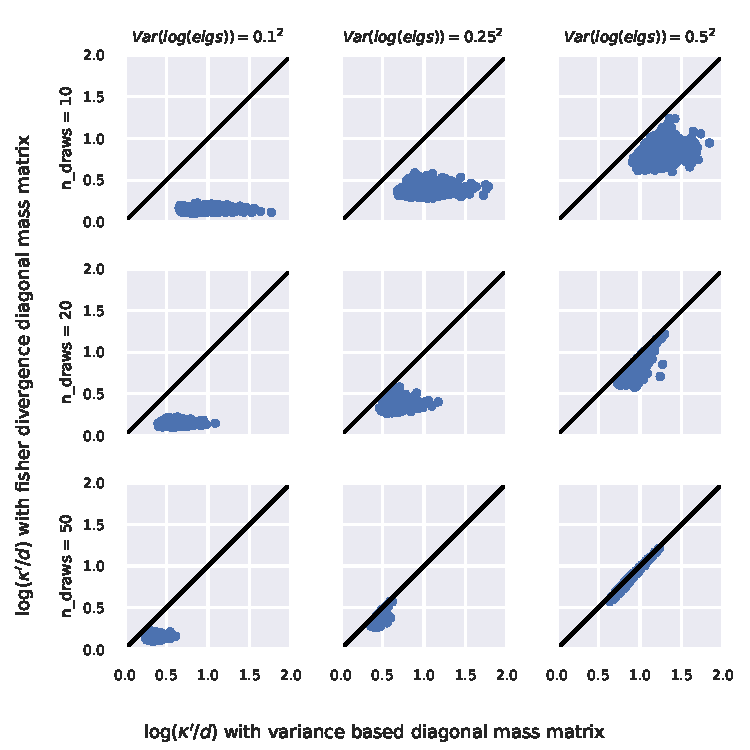
\includegraphics[width=0.35\textwidth]{img/diag_condition_number3.pdf}
\end{center}

\sld{Online Nutpie}
\begin{itemize}
\item Nutpie \myemph{cannot converge} with a fixed window of size $N=100$
\item Stan converges due to \myemph{exponentially increasing} blocksizes, e.g., $N
  = 20, 40, 80, \ldots$
\item \myemph{Online Nutpie} discounts past to mimic Stan:
  $\lambda_n = 1 / (\textrm{offset} + n)$
  \begin{subitemize}
  \item default $\textrm{offset} = 4$ reduces early variance
  \end{subitemize}
\item Compute \myemph{weighted means} and \myemph{weighted variances}:
  \begin{subitemize}
\item $\textrm{count}(n) = \lambda_n \cdot \textrm{count}(n-1) + 1$
\item $\textrm{mean}(n) = \left(\lambda_n \cdot \textrm{mean}(n-1) +
    \drw{\theta}{n}\right) / \textrm{count}(n)$
\item $\textrm{var}(n)$ same idea, weighted sum of square diffs from mean
\end{subitemize}
\vfill
\item Implement in \myemph{constant time} per iteration w.\
  \myemph{weighted Welford algorithm}
\end{itemize}

\sld{Initial inverse mass matrix}
\begin{itemize}
\item Stan initializes with \myemph{unit} inverse mass matrix.
\item Nutpie initializes with an approximation
\item For $\Theta \sim \textrm{normal}(\mu, \Sigma)$, $\mathbb{E}[S(\Theta) \cdot S(\Theta)^\top] =
  \Sigma$ (Fisher information)
\item Use \myemph{one-sample MCMC} approximation (or more)
\item If $\drw{\theta}{0}$ is initialization,
  $$
  M(0) = S(\drw{\theta}{0}) \, S^\top(\drw{\theta}{0})
  $$
\item Much \myemph{more effective} than unit in practice.
\end{itemize}

  

\sld{Discount schedule; {\normalsize $\textrm{offset} = 4$}}
\begin{center}
   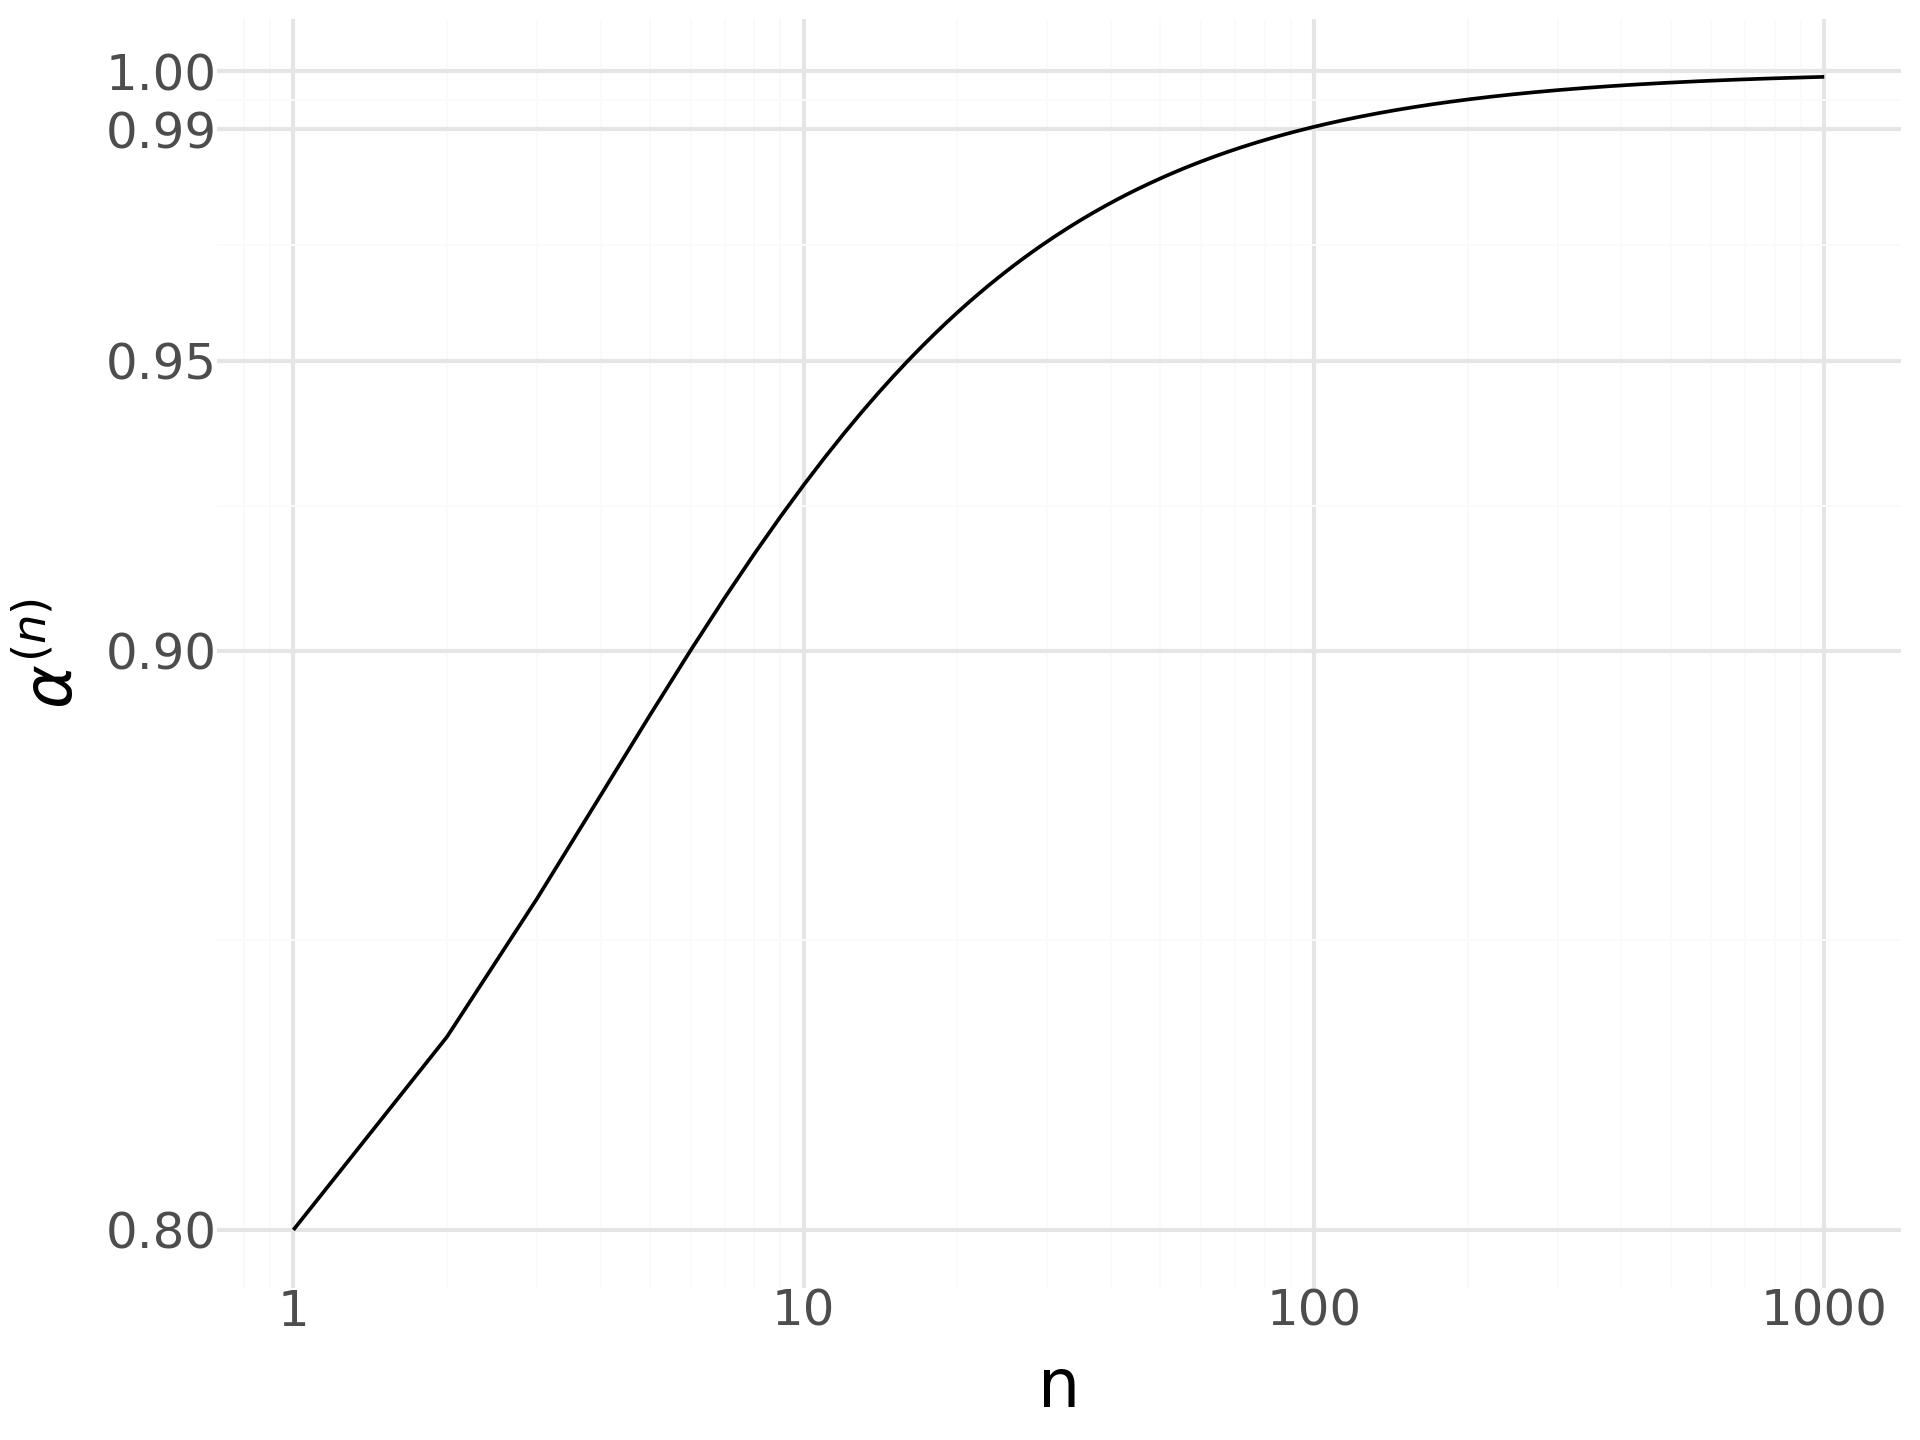
\includegraphics[width=0.6\textwidth]{img/discount-schedule.jpg}
 \end{center}

\sld{Performance: {\normalsize $\textrm{normal}(\theta \mid 0, \, \textrm{diagMat}([1, 2, 4, \ldots, 200]))$}}
\begin{center}
  \begin{center}
    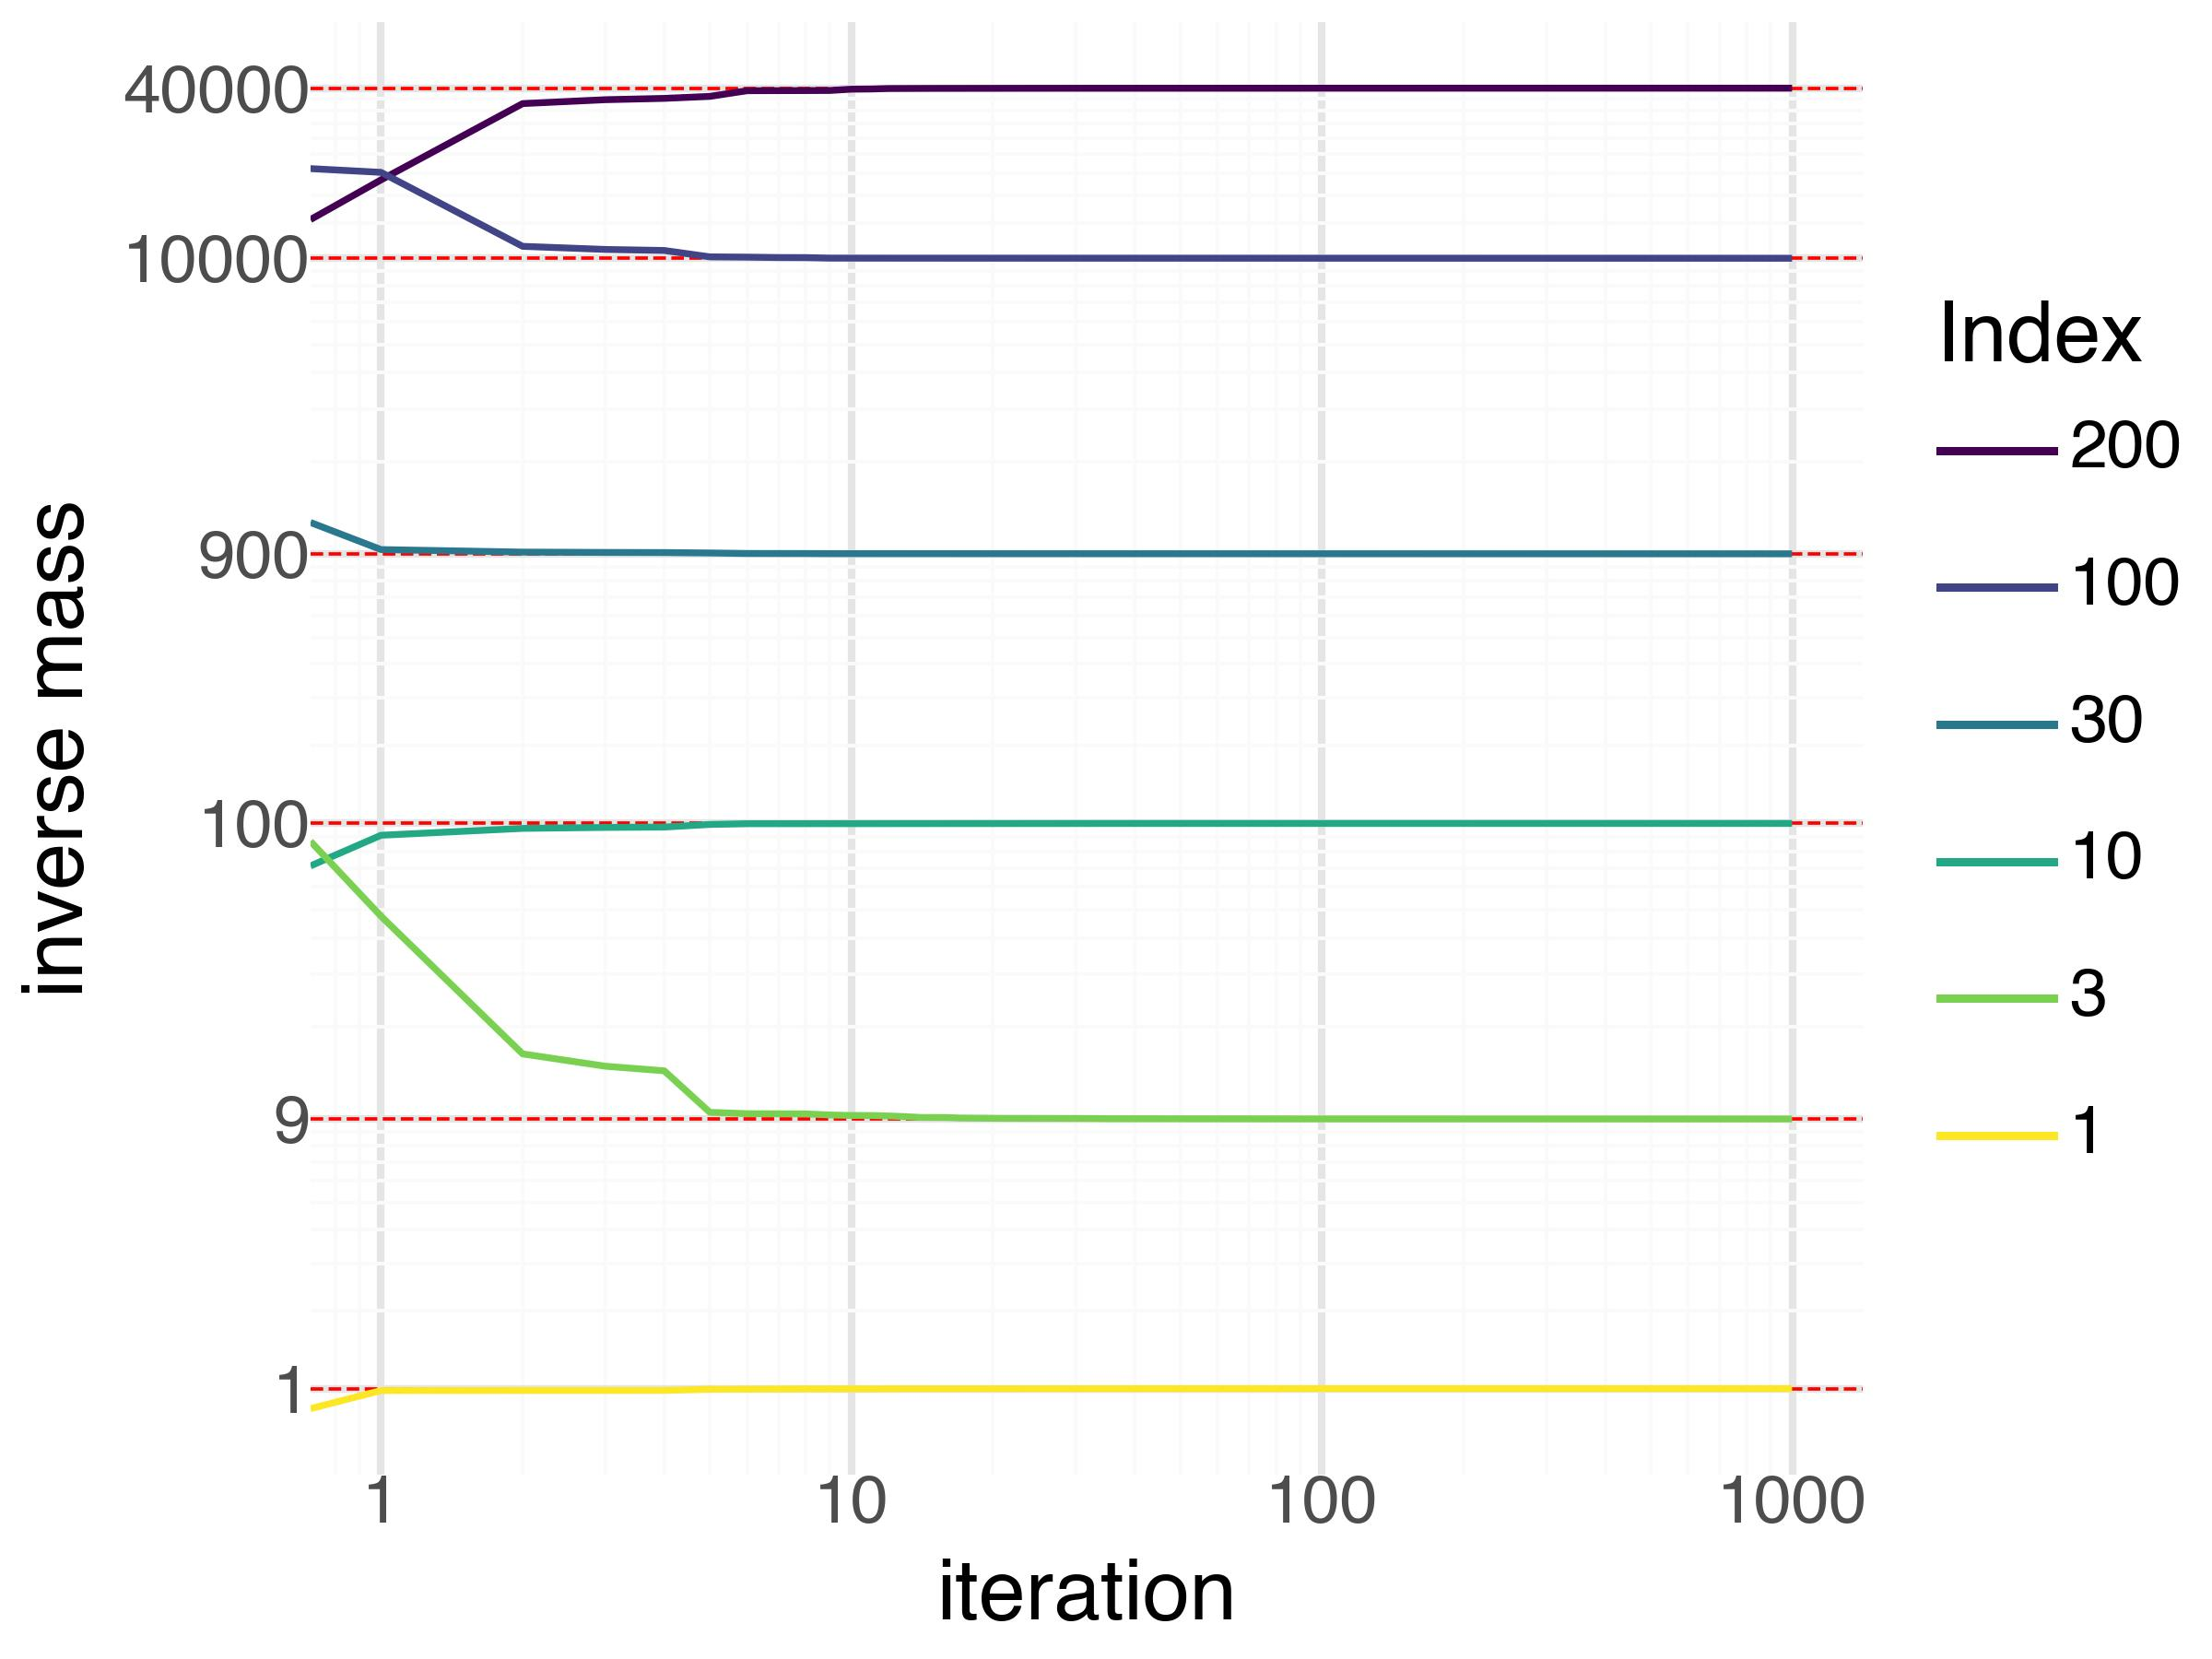
\includegraphics[width=0.45\textwidth]{img/walnuts-warmup-inv-mass.jpg}
  \end{center}
  \begin{itemize}
  \item \myemph{Converges} in \myemph{10 iterations}!
  \end{itemize}
\end{center}

\sld{Step-size tuning via SGD}
\begin{itemize}
\item Tuning parameter: \myemph{target acceptance rate} $\rho \in (0,
  1)$
\item Acceptance rate \myemph{monotonic} in step size (lower step,
  higher accept)
\item \myemph{Observed acceptance rate} $\alpha_n \in (0, 1)$ at MCMC step $n$
\item \myemph{Quadratic loss}: $\textrm{loss}_\rho(\alpha_n) =
  \frac{1}{2} (\alpha_n - \rho)^2$
\item Given \myemph{observed acceptance} $\alpha_n$ stochastic
  gradient is
  $$\nabla \textrm{loss}_\rho(\alpha_n) = \alpha_n - \rho$$
\end{itemize}

\sld{SGD algorithms: Adam vs.\ Dual averaging}
\begin{itemize}
\item SGD algorithm is \myemph{modular}, thus easy to swap
\item NUTS used \myemph{dual averaging}; 2010 state of the art
  \begin{subitemize}
    \item dual averaging uses stochastic mean to reduce variance
  \end{subitemize}
\item WALNUTS uses \myemph{Adam}; 2023 state of the art SGD
  \begin{subitemize}
    \item Adam estimates a regularized ``momentum'' for acceleration
    \end{subitemize}
\item For (WAL)NUTS, Adam is \myemph{faster to converge} and
  \myemph{lower variance} 
  \begin{subitemize}
  \item even w.\ Matt Hoffman's \myemph{regularization hack} of dual averaging for NUTS
  \end{subitemize}
\vfill
\item \myemph{Muon} may be the 2026 state-of-the-art SGD
\end{itemize}

\sld{Adam faster, more stable}
\begin{center}
  \spc
    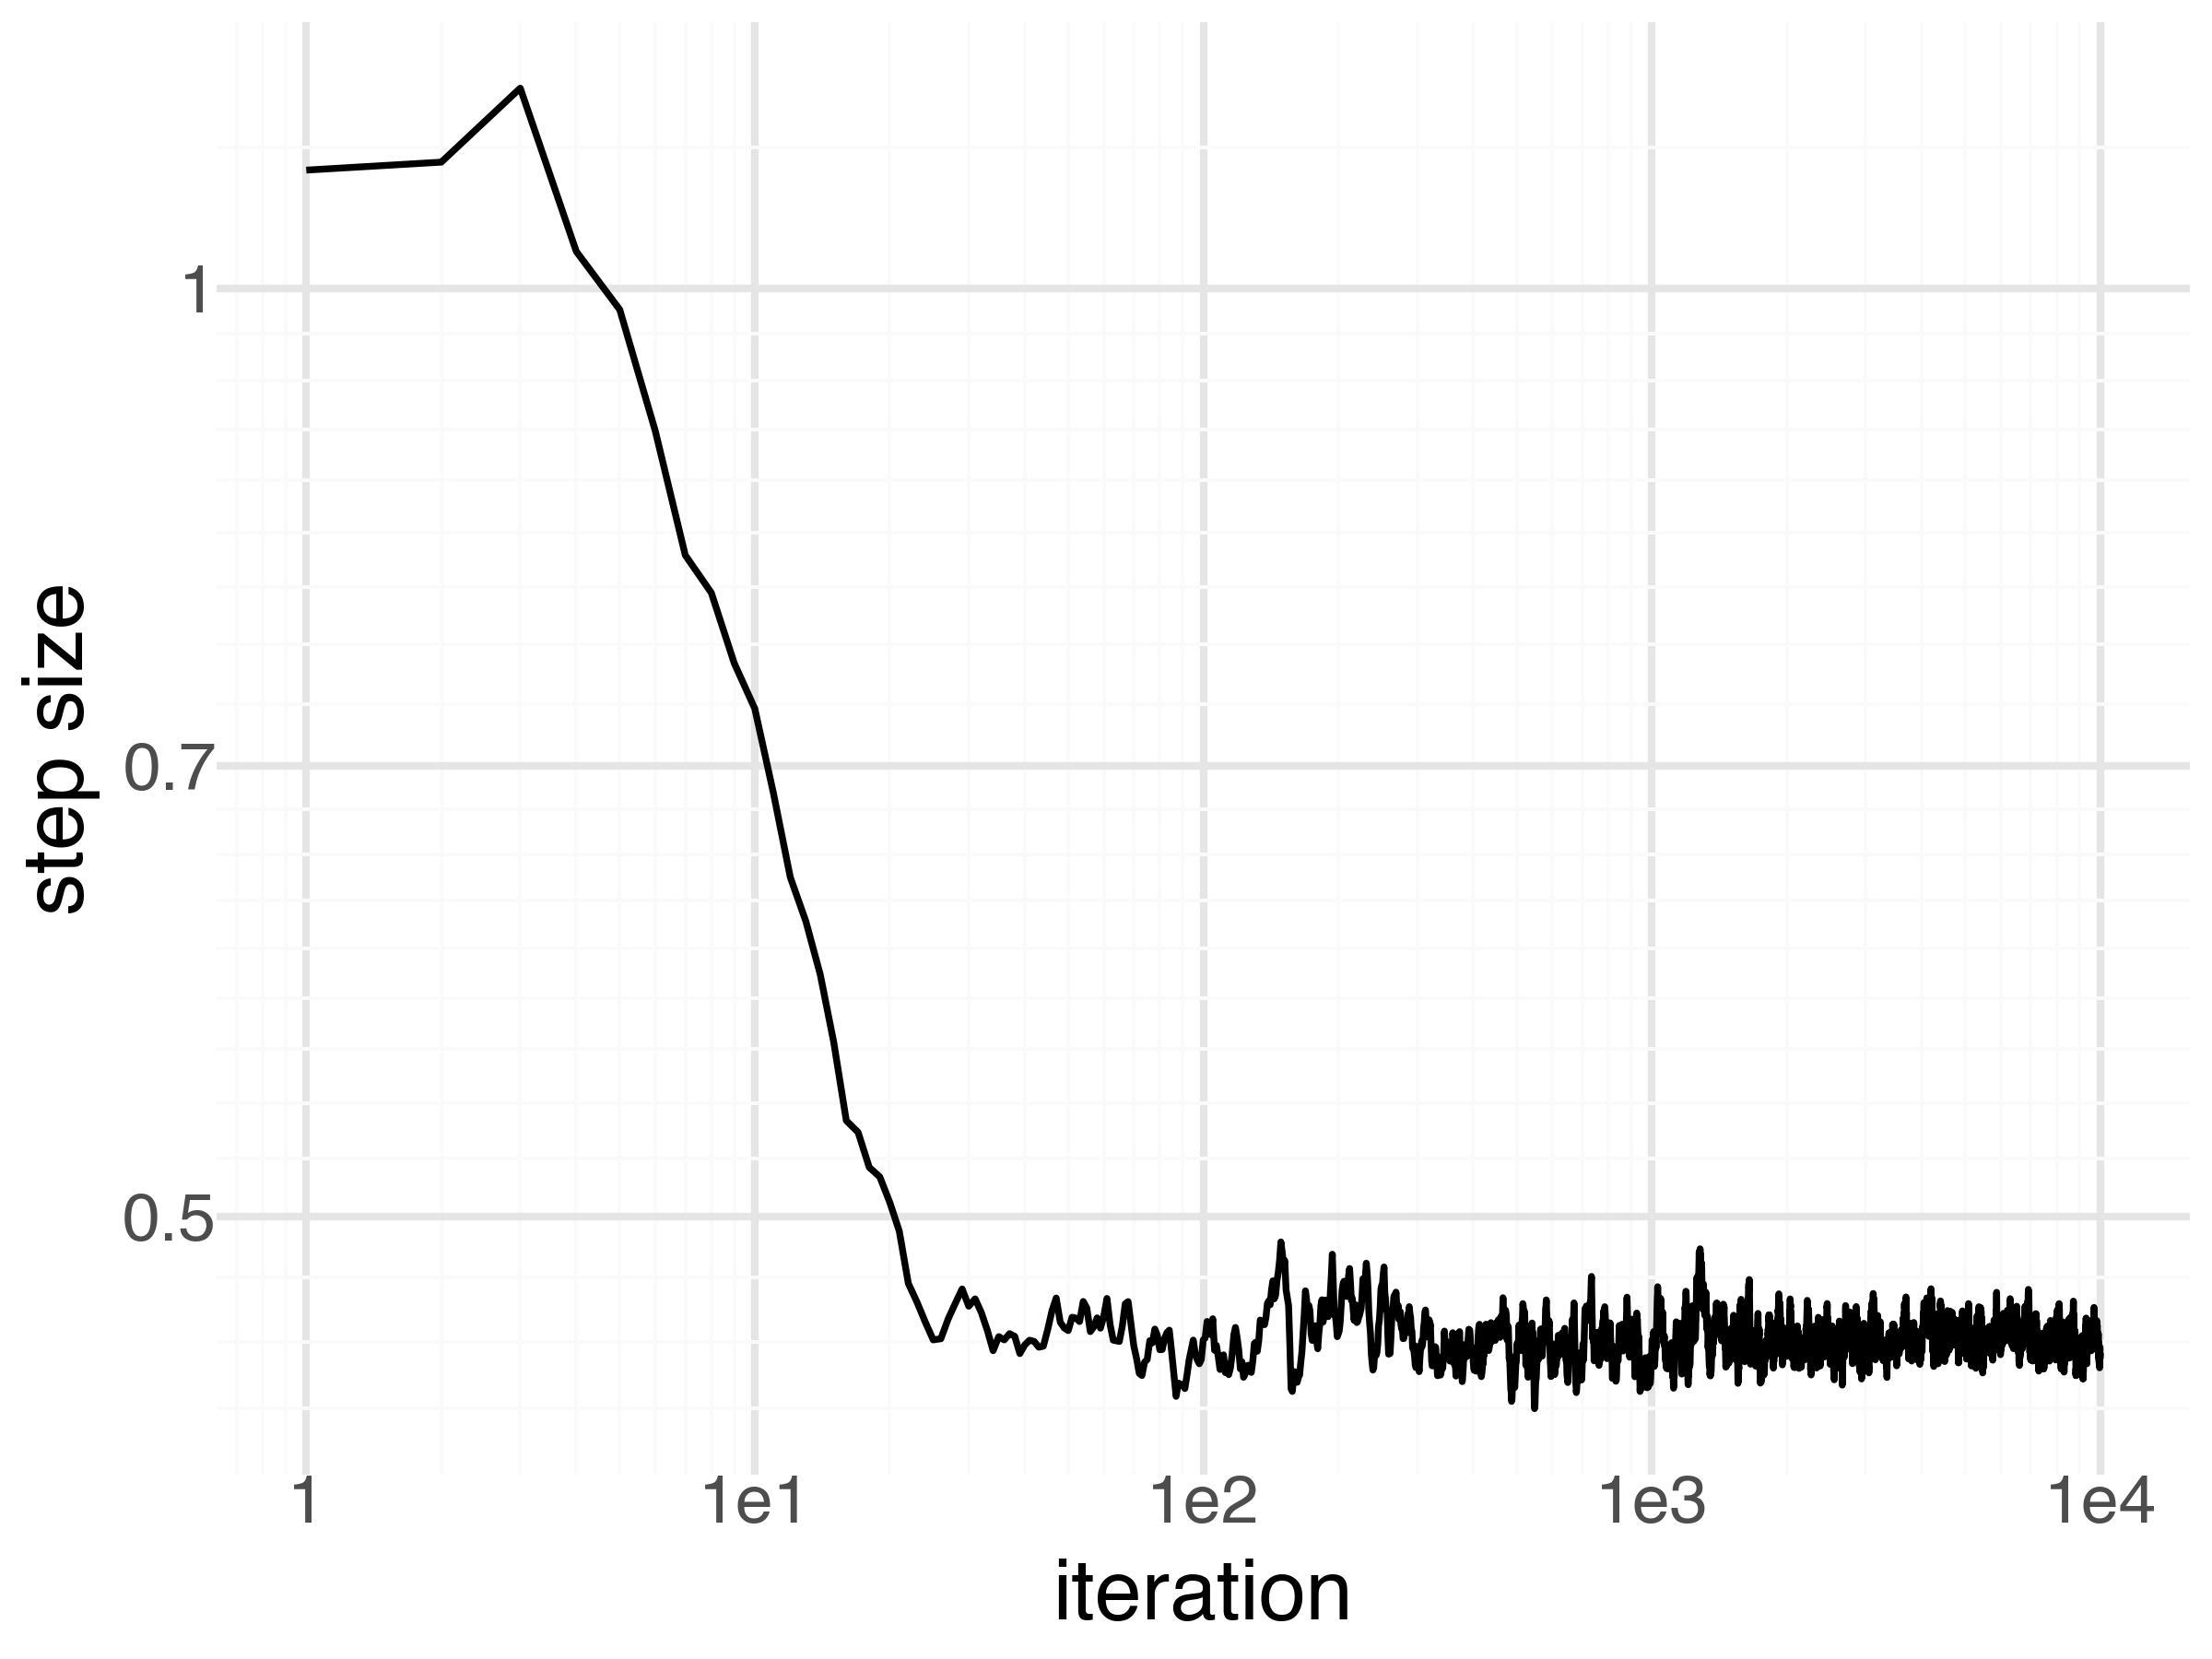
\includegraphics[width=0.4\textwidth]{img/adam-step-warmup.jpg}
    \hfill
    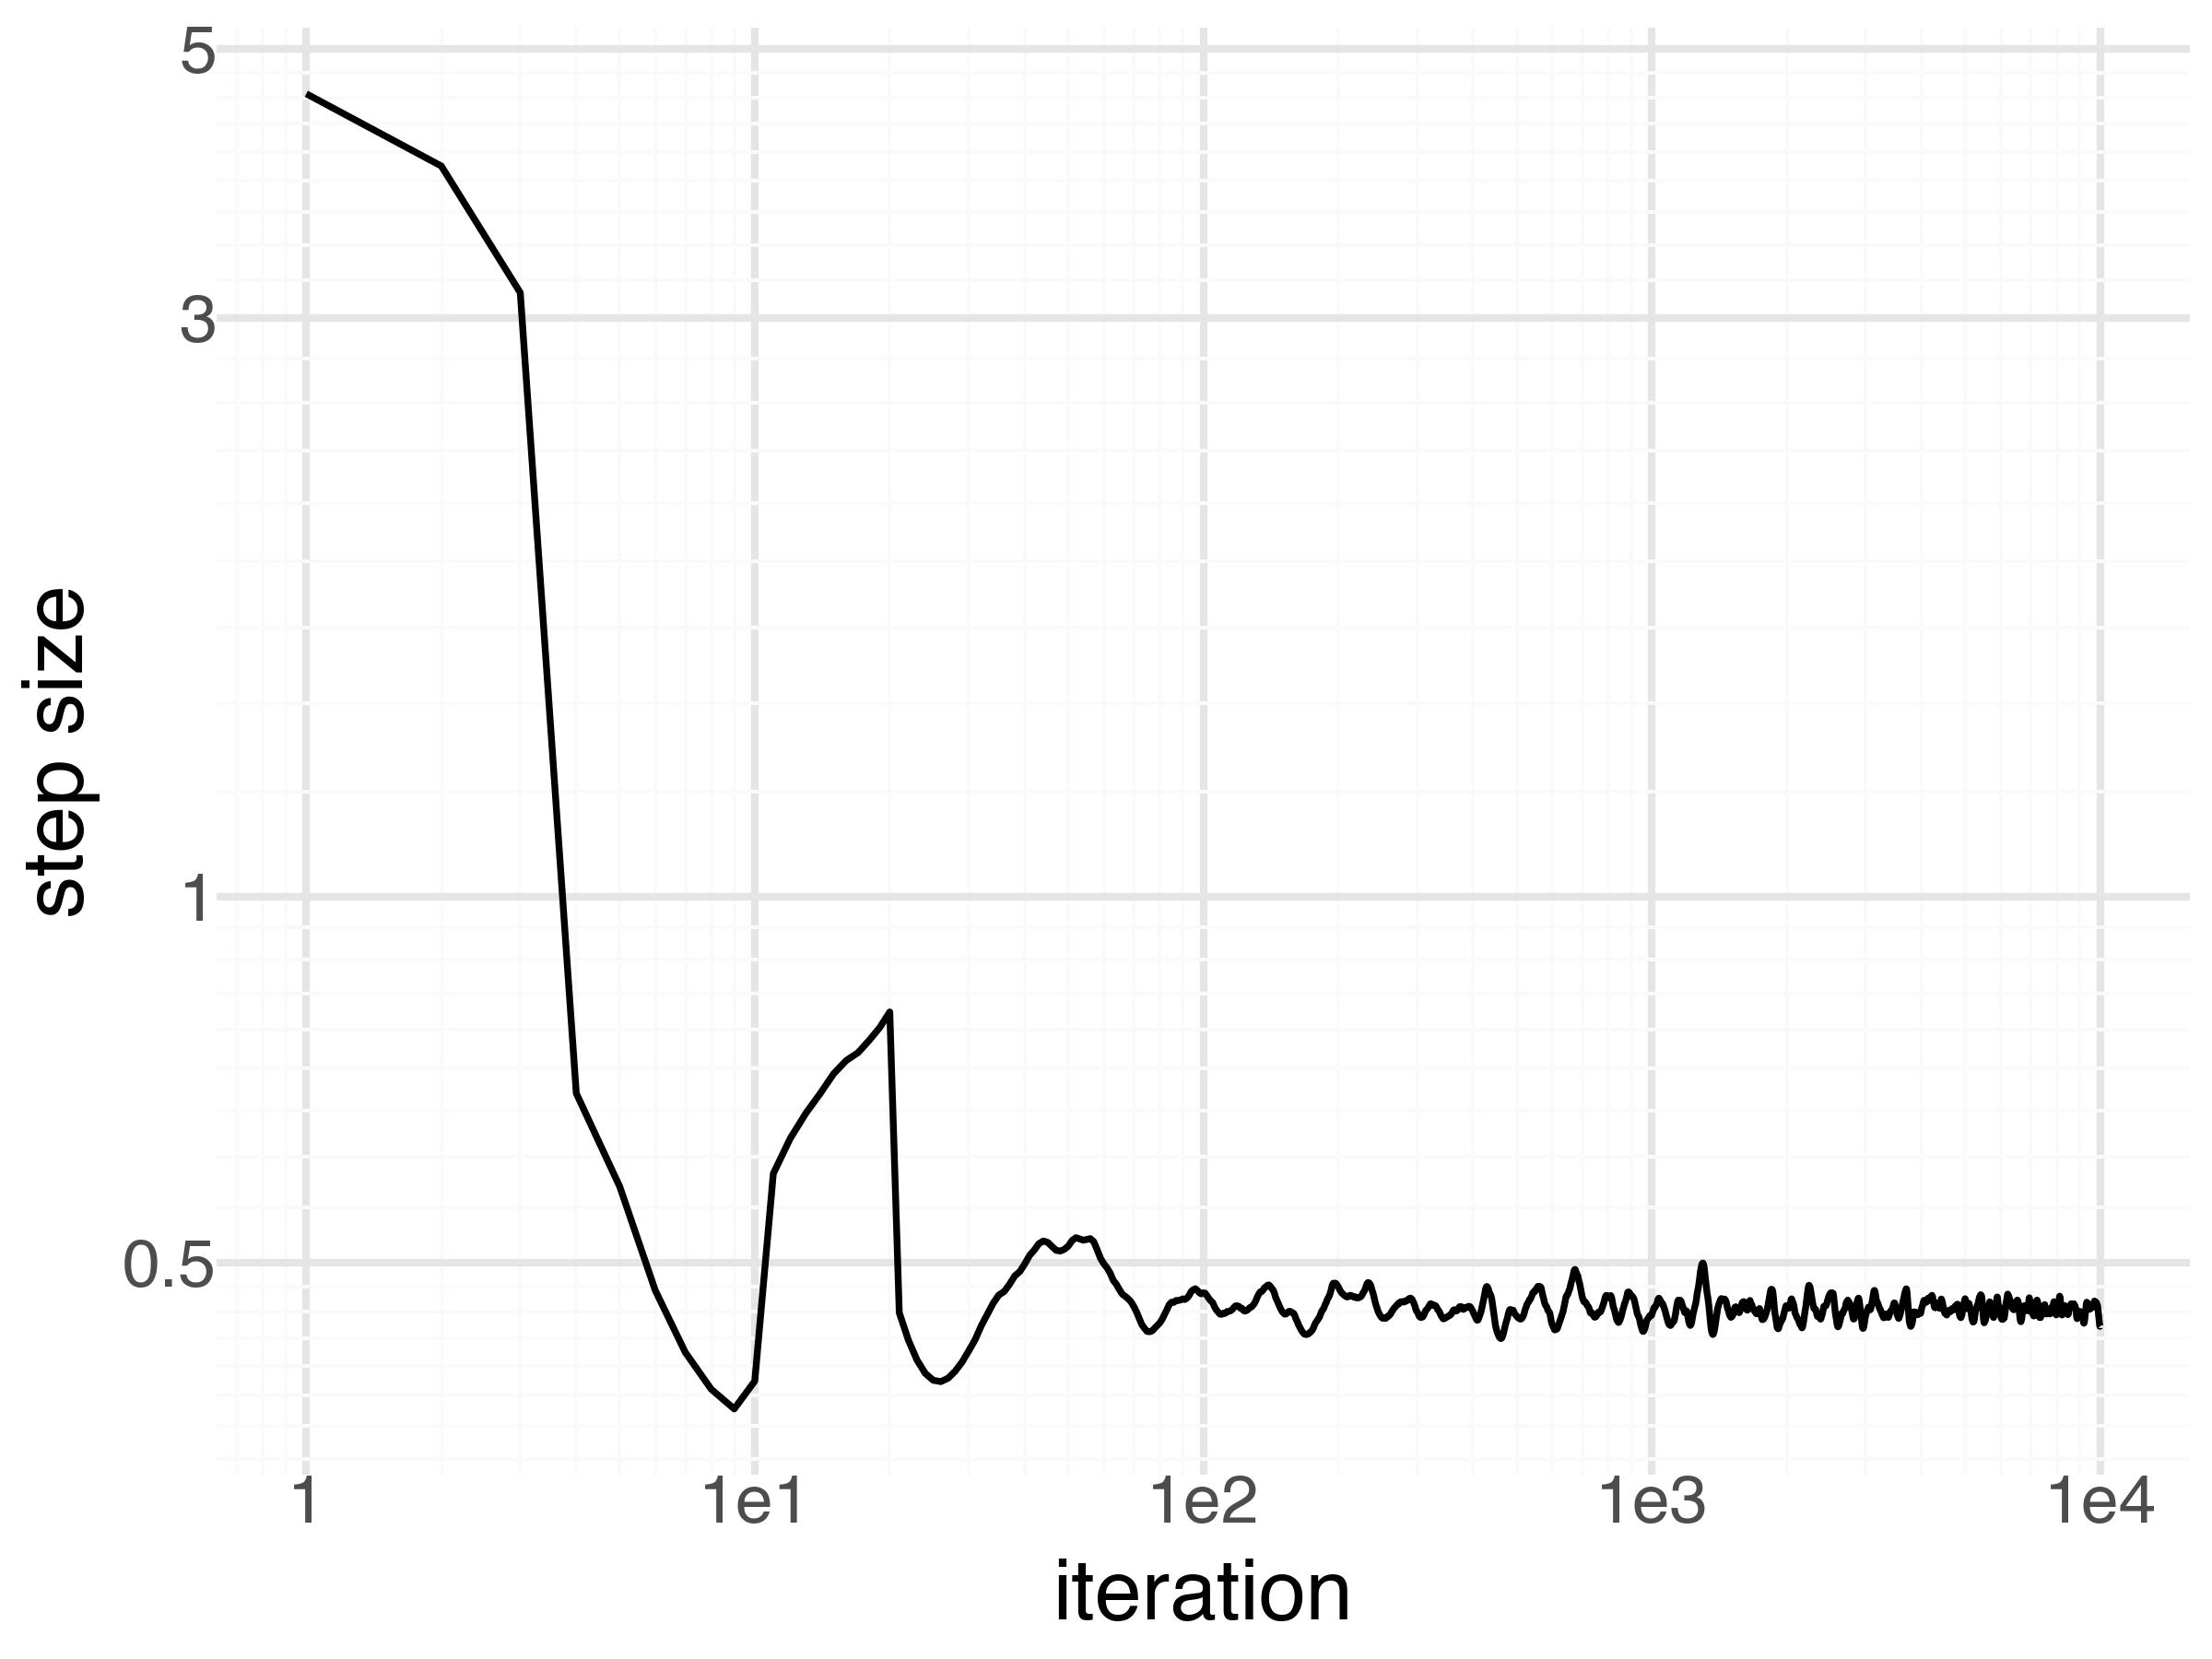
\includegraphics[width=0.4\textwidth]{img/dual-avg-step-warmup.jpg}
  \end{center}
\begin{subitemize}
\item \myemph{log scale} $x$-axis and $y$-axis; \myemph{different
    ranges} on $y$-axis (1 vs.\ 5)
\item Faster step adapt accelerates \myemph{burn-in} and \myemph{mass matrix adaptation}.
\end{subitemize}


\sld{Lock-free, parallel convergence monitoring}
\begin{itemize}
  \item \myemph{$\widehat{R}$ statistic} converges to 1 for chains with same
    stationary distribution
  \item \myemph{One chain per thread} accumulating mean and variance
    using Welford
  \item \myemph{SPSC parallelism}: single producer (chain), single consumer (monitor)
  \item \myemph{Monitor thread} reads mean/variance/count from chains
  \item Monitor computes $\widehat{R}$; terminates chains if below threshold
    threshold.
  \item SPSC implemented with \myemph{lock-free atomics}
    (\texttt{std::atomic}) in C++11x
    \begin{subitemize}
    \item mean/variance/count packed single precision in 12 bytes
    \end{subitemize}
  \item Monitor \myemph{only log density} $\log p(\theta)$---usually
    slower than single parameters
\end{itemize}

\sld{Lock-free, parallel adaptation monitoring}
\begin{itemize}
\item We're adapting a \myemph{step size} (scalar) and a \myemph{diagonal mass matrix}
  (vector).
\item Use a \myemph{triple buffer} for lock-free SPSC parallelism
  queue.
\item \myemph{Step size convergence} if each chain's step size is
  within tolerance of the geometric mean across chains.
\item \myemph{Mass matrix convergence} if each chain's standardized
  (vs. geometric mean) L2 norm is within tolerance of the geometric
  mean of chains
  \vfill
\item \myemph{No measurable overhead} on my Mac Studio
  \begin{subitemize}
    \item M3-ultra CPU; 20 performance cores; 256 GB
      \myemph{integrated RAM}
    \item \myemph{Mac ARM 5+ times faster} than Intel for \myemph{memory-intensive
      parallelism}
  \end{subitemize}
\end{itemize}


  
\sld{Collaborators and references}
\begin{subitemize}
\item \myemph{WALNUTS GitHub}: \texttt{flatironinstitute/walnuts}
\item \myemph{Nutpie GitHub}:  \texttt{pymc-devs/nutpie}
\item Nawaf Bou-Rabee, Bob Carpenter, Tore Kleppe, Sifan Liu.
      2026. \myemph{WALNUTS: The within-orbit adaptive leapfrog no-U-turn
        sampler}. {\slshape JMLR} ({\slshape arXiv} 2506.18746).
    \item Adrian Seyboldt, Eliot Carlsen, Bob Carpenter. 2026. \myemph{Preconditioning Hamiltonian Monte
Carlo by minimizing Fisher Divergence}. In progress.
\end{subitemize}
\spc
\begin{tabular}{cccccc}

\includegraphics[height=0.15\textwidth]{img/nawaf.jpg}
&

\includegraphics[height=0.15\textwidth]{img/tore.png}
&

\includegraphics[height=0.15\textwidth]{img/sifan.jpg}
  &
    \hspace*{18pt}
    & 
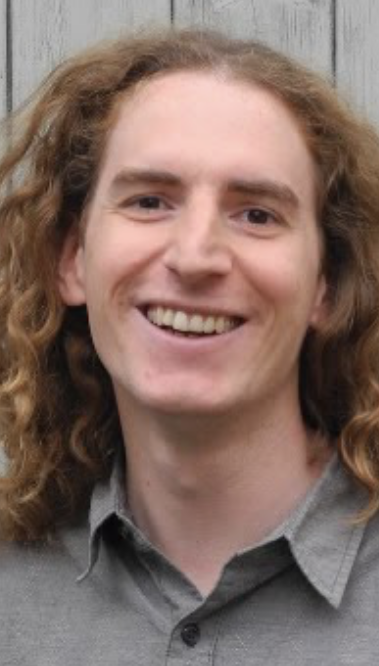
\includegraphics[height=0.15\textwidth]{img/adrian-seyboldt.png}
&
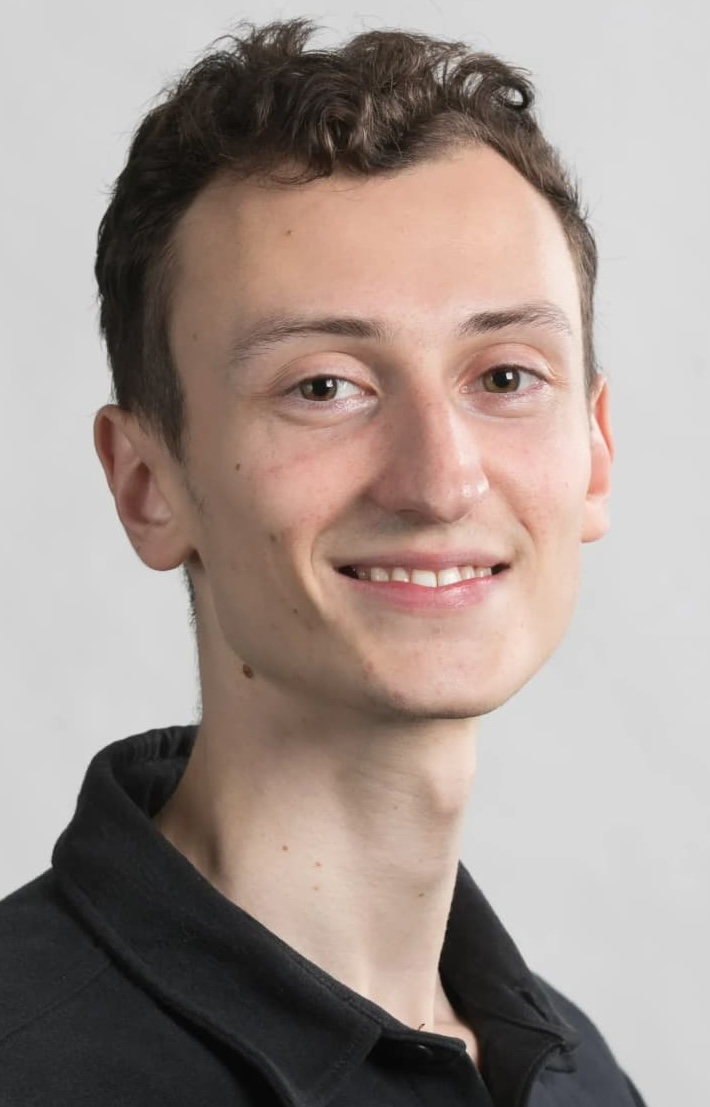
\includegraphics[height=0.15\textwidth]{img/eliot-carlsen.jpg}
\\
Bou-Rabee & Kleppe & Liu & & Seyboldt & Carlsen
\end{tabular}


\end{document}